\documentclass[a4paper,11pt]{article}

%%%%%%%%%%%%%%%%%%%%%%%%%%%%%%%%%%%%%%%%%%%%%%%%%%%%%%%%%%%%%%%%%%%%%%%%
% Paquetes utilizados
%%%%%%%%%%%%%%%%%%%%%%%%%%%%%%%%%%%%%%%%%%%%%%%%%%%%%%%%%%%%%%%%%%%%%%%%

\usepackage[margin=0.8in]{geometry}

% Gráficos complejos
\usepackage{graphicx}
\usepackage{caption}
\usepackage{subcaption}
\usepackage{placeins}

% Soporte para el lenguaje español
\usepackage{textcomp}
\usepackage[utf8]{inputenc}
\usepackage[T1]{fontenc}
\DeclareUnicodeCharacter{B0}{\textdegree}
\usepackage[spanish]{babel}

% Código fuente embebido
\usepackage{listings}
\usepackage{courier}

% PDFs embebidos para el apéndice
\usepackage{pdfpages}

% Matemáticos
\usepackage{amssymb,amsmath}

% Tablas complejas
\usepackage{multirow}

% Formato de párrafo
\setlength{\parskip}{1ex plus 0.5ex minus 0.2ex}

% Subrayado de palabras
\usepackage[normalem]{ulem}

% Formato de listados de código
\lstset{
  basicstyle=\footnotesize\ttfamily,
  numberstyle=\tiny,
  numbersep=5pt,
  tabsize=2,
  extendedchars=true,
  breaklines=true,
  stringstyle=\color{white}\ttfamily,
  showspaces=false,
  showtabs=false,
  xleftmargin=17pt,
  framexleftmargin=17pt,
  framexrightmargin=5pt,
  framexbottommargin=4pt,
  showstringspaces=false,
  language=SQL
}
\usepackage{caption}
\DeclareCaptionFont{white}{\color{white}}
\DeclareCaptionFormat{listing}{\colorbox[cmyk]{0.43, 0.35, 0.35,0.01}{\parbox{\textwidth}{\hspace{15pt}#1#2#3}}}
\captionsetup[lstlisting]{format=listing,labelfont=white,textfont=white, singlelinecheck=false, margin=0pt, font={bf,footnotesize}}

%%%%%%%%%%%%%%%%%%%%%%%%%%%%%%%%%%%%%%%%%%%%%%%%%%%%%%%%%%%%%%%%%%%%%%%%
% Título
%%%%%%%%%%%%%%%%%%%%%%%%%%%%%%%%%%%%%%%%%%%%%%%%%%%%%%%%%%%%%%%%%%%%%%%%

% Título principal del documento.
\title{\textbf{Trabajo Práctico: Cotizador de pólizas}}

% Información sobre los autores.
\author{
  Gabriel Jaimerena,      \textit{P. 83.375},	\textit{gabrieljaimerena@gmail.com}	            \\
  Lorena Kalaydjian,     \textit{P. 81.925},	\textit{lorenak@gmail.com}                		\\
  Sergio Matías Piano,     \textit{P. 85.191},	\textit{smpiano@gmail.com}                  	\\
  Javier Daniel Zaniratto, \textit{P. 90.886},	\textit{jzaniratto@fi.uba.ar}                   \\
  \\
  \normalsize{Grupo 16}                        			  			\\
  \normalsize{2do. Cuatrimestre de 2013}                           	\\
  \normalsize{75.15 - Bases de datos}                              	\\
  \normalsize{Facultad de Ingeniería, Universidad de Buenos Aires}
}
\date{}

%%%%%%%%%%%%%%%%%%%%%%%%%%%%%%%%%%%%%%%%%%%%%%%%%%%%%%%%%%%%%%%%%%%%%%%%
% Documento
%%%%%%%%%%%%%%%%%%%%%%%%%%%%%%%%%%%%%%%%%%%%%%%%%%%%%%%%%%%%%%%%%%%%%%%%

\begin{document}

% ----------------------------------------------------------------------
% Top matter
% ----------------------------------------------------------------------
\thispagestyle{empty}
\maketitle

\begin{abstract}

  Este informe resume el desarrollo del trabajo práctico de la materia Base
  de Datos (75.15) dictada en el segundo cuatrimestre de 2013 en la Facultad de
  Ingeniería de la Universidad de Buenos Aires. El mismo consiste en el
  modelado de datos de un software de cotización de pólizas de automotor y otros riesgos,
  cuyos requisitos fueron extraído de un caso de estudio real.

\end{abstract}

\clearpage

% ----------------------------------------------------------------------
% Tabla de contenidos
% ----------------------------------------------------------------------
\tableofcontents
\clearpage


% ----------------------------------------------------------------------
% Desarrollo
% ----------------------------------------------------------------------
\part{Desarrollo}


\section{Modelo de entidad-interrelación} \label{sec:der}

\subsection{Hipótesis}

\begin{enumerate}
 
	\item La entidad Inspección es "débil" de cotizacción, ya que cada cotización tendrá inspeccionar con nroInspeccion 1, 2, 3, etc..
 
	\item La entidad Sucursal posee el dato de todas las sucursales y la Casa central inclusive.

	\item Se asume que el cliente que solicita la cotización y es aprobada es titular del vehículo
	
	\item El vehículo a ser asegurado tiene la VTV vigente.

	\item El re-aseguro y co-aseguro, atributos de la cobertura indican que fue revisado por las entidades correspondientes (nacional o bien extranjera) y que la cobertura contempla la modificación.

	\item La tasa fija de las cuotas está considerada dentro del monto.

	\item Puede haber sucursales que aún no hayan podido generar una cotización.

	\item Los ejecutivos de cuenta de la casa central pueden tener que analizar o no la solicitud de cotización.  

	\item La entidad Cotización tendrá los datos sobre el plan de cuotas, y la entidad débil Cuotas registrará los datos de cada una.
 
	\item La entidad Rubro abarca todos los tipos de rubros, no se usará herencia para poner los distintos tipos por simpleza del diagrama, por lo tanto, se sobreentiende que debería existir una entidad por cada tipo distinto de rubro pero se obviarán.
	
	\item El productor se seguros calcula la prima y monto de la solicitud de cobertura utilizando una planilla excel o un cotizador online que está disponible solo para los productores y empleados de la compañía.
  
\end{enumerate}


\subsection{Diagrama de entidad-interrelación}

 En la figura \ref{fig:der} se incluye el diagrama de entidad-interrelación
 final desarrollado para representar el dominio modelado cuyo relevamiento se
 detalla en el enunciado.

\begin{figure}[h!t]
  \centering
  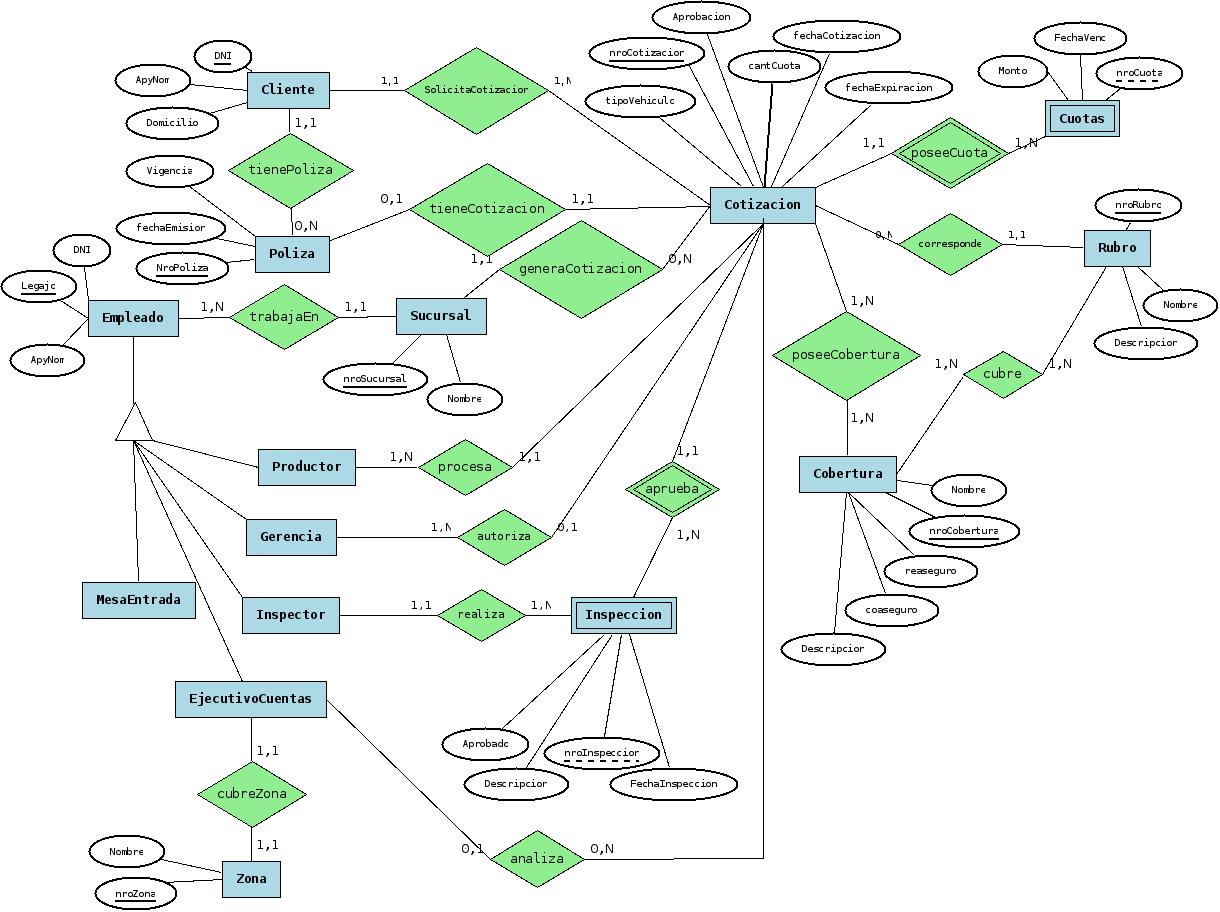
\includegraphics[width=1.4\textwidth, angle=90]{build/images/der.jpeg}
  \caption{Diagrama de entidad-interrelación} \label{fig:der}
\end{figure}

\FloatBarrier


\subsection{Dependencias de identidad y de existencia}

\begin{itemize}

  \item \textbf{Cotizacion - Sucursal}	Dependencia de existencia	
  
  \item \textbf{Cotizacion - Cliente}	Dependencia de existencia	

  \item \textbf{Cotizacion - Rubro}	Dependencia de existencia	

  \item \textbf{Cuotas - Cotizacion}	Dependencia de existencia e identidad

  \item \textbf{Empleado - Sucursal}	Dependencia de existencia	

  \item \textbf{Inspeccion - Inspector}	Dependencia de existencia	

  \item \textbf{Inspeccion - Cotizacion}	Dependencia de existencia e identidad 

  \item \textbf{Poliza - Cliente}	Dependencia de existencia	

  \item \textbf{Poliza - Cotizacion}	Dependencia de existencia	

  \item \textbf{Productor - Cotizacion}	Dependencia de existencia	

\end{itemize}

\section{Diccionario de datos}

\subsection{Cliente}

Representa las distintas personas físicas que solicitarán cotizaciones para asegurar 
a sus distintos vehículos.

\begin{itemize}

  \item \textbf{\uline{dni}} Clave que identifica a un cliente.
  
  \item \textbf{apellido} Apellidos del cliente.

  \item \textbf{nombre} Nombres del cliente.
  
  \item \textbf{domicilio} Lugar donde reside el cliente.
  
  \item \textbf{telefono} Número telefónico para contactar al cliente.
  
  \item \textbf{email} E-mail para contactar al cliente.
  
\end{itemize}

\subsection{SolicitaCotización}

Relaciona los clientes con las distintas cotizaciones solicitadas.

\subsection{Cotización}

Representa las distintas formas de asegurar un vehículo que los clientes recibirán para poder asegurar
un vehículo.

\begin{itemize}

  \item \textbf{\uline{nroCotizacion}} Número único e identificatorio de cada cotización.
  
  \item \textbf{tipoVehiculo} Almacena el tipo de vehículo para el cual la cotización ha sido generada.

  \item \textbf{fechaExpiracion} Fecha en la cual deja de tener validez ésta cotización.
  
  \item \textbf{cantCuota} Cantidad de cuotas.

  \item \textbf{fechaCotizacion} Fecha en la cual se ha realizado la cotización.
      
\end{itemize}

\subsection{PoseeCuota}

Interrelación entre las cotizaciones y cada cuota de su plan de pago.

\subsection{Cuota}

Indica las distintas cuotas que se deben pagar para la cotización en caso de contratarla.

\begin{itemize}

  \item \textbf{\dashuline{nroCuota}} Número de cuota del pago.
    
  \item \textbf{\uline{idCotizacion}} Número único e identificatorio de cada cotización.
  
  \item \textbf{monto} Suma de dinero que se deberá pagar en una determinada cuota.

  \item \textbf{fechaVencimiento} Fecha hasta la cual dse puede realizar el pago.

\end{itemize}

\subsection{TienePoliza}

Relación entre cada cliente y sus pólizas solicitadas.

\subsection{TieneCotización}

Une a las distintas pólizas con su cotización correspondiente.

\subsection{Póliza}

Los distintos seguros que contrató cada cliente.

\begin{itemize}
   
  \item \textbf{\uline{nroPoliza}} Número único e identificatorio de cada póliza.
  	
  \item \textbf{fechaEmision} Indica la fecha en la cuál empieza a tomar vigencia la póliza.
      
\end{itemize}

\subsection{GeneraCotizacion}

Nos permite obtener las cotizaciones generadas por cada sucursal.

\subsection{Sucursal}

Las distintas sucursales en las que los clientes podrán solicitar cotizaciones para asegurar sus vehículos

\begin{itemize}
   
  \item \textbf{\uline{nroSucursal}} Número que identifica a una sucursal.
  
  \item \textbf{nombre} Nombre de la sucursal.
  
\end{itemize}

\subsection{TrabajaEn}

Relaciona a cada empleada con la sucursal en la cual trabaja.

\subsection{Empleado}

Representa los trabajadores que realizarán las tareas necesarias para generarle cotizaciones
a los distintos clientes.

\begin{itemize}
   
  \item \textbf{\uline{legajo}} Número interno que representa a cada empleado.
  
  \item \textbf{dni} Documento de indentidad del empleado.
  
  \item \textbf{nombre} Nombre del empleado.
  
  \item \textbf{apellido} Apellidos del empleado.
  
\end{itemize}

%\subsection{Rol}

%Representa los distintos puestos de trabajo en el que un empleado puede trabajar.

%\begin{itemize}
   
%  \item \textbf{\uline{NroRol}} Número identificatorio de cada rol.
  
%  \item \textbf{Nombre} Nombre descriptivo del rol.
  
%\end{itemize}

\subsection{Mesa de entradas}

Representa a los empleados que recibirán las solicitudes para asegurar.

\subsection{Ejecutivo de cuenta}

Empleados que analizarán en casos especiales las cotizaciones.

\subsection{Analiza}

Relaciona las distintas cotizaciones con quien la analizó o no.

\subsection{Productor}

Empleados que procesarán las distintas cotizaciones.

\subsection{Procesa}

Almacena qué empleados procesaron cada cotización.

\subsection{Gerencia}

Empleados que autorizarán las distintas cotizaciones.

\subsection{Autoriza}

Relaciona las distintas cotizaciones con el o los empleados que la han autorizado.

\subsection{Inspector}

Empleados que realizarán inspecciones para determinar 
la aprobación o no de las cotizaciones.

\subsection{Realiza}

Relación que nos permitirá saber qué inspector realizó cada inspección.

\subsection{Inspección}

Representa las distintas inspecciones que los inspectores realizarán para aprobar o no las cotizaciones.
Cada inspección conecta a una cotización con el inspector que la inspeccionó.

\begin{itemize}
   
  \item \textbf{\dashuline{nroInspeccion}} Número de inspección que realiza un inspector dado a una cotización.
  
  \item \textbf{\uline{idCotizacion}} Id de la cotización para la que se realiza dicha inspección.
    
  \item \textbf{descripcion} Mensaje indicando las observaciones de la inspección.

  \item \textbf{aprobado} Indica si fue aprobada la cotización.
    
\end{itemize}

\subsection{Aprueba}

Nos permité conocer en qué inspección ha sido aprobada cierta cotización.

\subsection{Zona}

Son las distintas zonas que cubrirán los ejecutivos de cuenta.

\begin{itemize}
   
  \item \textbf{\uline{idZona}} Número identificatorio de cada zona.
  
  \item \textbf{nombre} Nombre descriptivo de la zona.
  
\end{itemize}

\subsection{CubreZona}

Qué zona cubre cada ejecutivo de cuentas.

\subsection{Rubro}

Representa las distintas categorías a la cual una cotización puede pertenecer.

\begin{itemize}
   
  \item \textbf{\uline{nroRubro}} Número identificatorio de cada rubro.
  
  \item \textbf{nombre} Nombre del rubro.

  \item \textbf{descripcion} Texto descriptivo del rubro.
  
\end{itemize}

\subsection{Corresponde}

Relaciona las cotizaciones con el rubro al cual pertenecen.

\subsection{Cubre}

Guardará qué rubros estarán contemplados en cada cobertura.

\subsection{Cobertura}

Son los riesgos que están cubiertos en una póliza según el rubro que corresponda.

\begin{itemize}
   
  \item \textbf{\uline{nroCobertura}} Número identificatorio de cada cobertura.
  
  \item \textbf{nombre} Nombre de la cobertura.

  \item \textbf{descripcion} Texto descriptivo de la cobertura.
  
  \item \textbf{reaseguro} Nombre de la compañía extranjera reaseguradora

  \item \textbf{coaseguro} Almacena si la cobertura tiene coaseguro con la empresa Aliance S.A.
  
\end{itemize}

\subsection{PoseeCobertura}

Almacenará las coberturas que tendrán las distintas cotizaciones.


\section{Modelo relacional}

\subsection{Claves candidatas}

\subsubsection{Cuotas}

\begin{itemize}

	\item \textbf{Atributos:} \{nroCuota, nroCotizacion, fechaVencimiento, monto\}

	\item \textbf{Clave Primaria:} \{nroCuota, nroCotizacion\}

	\item \textbf{Claves Foráneas:} \{nroCotizacion\}

	\item \textbf{Atributos que pueden ser nulos:} -
	
\end{itemize}

\subsubsection{Cliente}

\begin{itemize}

	\item \textbf{Atributos:} \{dni, apellido, nombre, domicilio, telefono, email\}

	\item \textbf{Clave Primaria:} \{dni\}

	\item \textbf{Claves Foráneas:} -

	\item \textbf{Atributos que pueden ser nulos:} -
	
\end{itemize}

\subsubsection{Póliza}

\begin{itemize}

	\item \textbf{Atributos:} \{nroPoliza, nroCotizacion, dni, fechaEmision, fechaVigencia\}

	\item \textbf{Clave Primaria:} \{nroPoliza\}

	\item \textbf{Claves Foráneas:} \{nroCotizacion\}, \{dni\}

	\item \textbf{Atributos que pueden ser nulos:} -
	
\end{itemize}

\subsubsection{Posee cobertura}

\begin{itemize}

	\item \textbf{Atributos:} \{nroCobretura, nroCotizacion\}

	\item \textbf{Clave Primaria:} \{nroCobretura, nroCotizacion\}
	
	\item \textbf{Claves Foráneas:} \{nroCobertura\}, \{nroCotizacion\}

	\item \textbf{Atributos que pueden ser nulos:} -
	
\end{itemize}

\subsubsection{Cobertura}

\begin{itemize}

	\item \textbf{Atributos:} \{nroCobertura, nombre, reaseguro, coseguro, descripcion\}

	\item \textbf{Clave Primaria:} \{nroCobertura\}
	
	\item \textbf{Claves Foráneas:} -

	\item \textbf{Atributos que pueden ser nulos:} \{reaseguro, coseguro\} 
	
\end{itemize}

\subsubsection{Cubre}

\begin{itemize}

	\item \textbf{Atributos:} \{nroRubro, nroCobertura\}

	\item \textbf{Clave Primaria:} \{nroRubro, nroCobertura\}
	
	\item \textbf{Claves Foráneas:} \{nroRubro\}, \{nroCobertura\}

	\item \textbf{Atributos que pueden ser nulos:} -
	
\end{itemize}


\subsubsection{Cotización}

\begin{itemize}

	\item \textbf{Atributos:} \{nroCotizacion, tipoVehiculo, cantCuotas, fechaCotizacion, fechaExpiracion, dni, nroRubro, legajo, nroSucursal, aprobacion\}
	
	\item \textbf{Clave Primaria:} \{nroCotizacion\}
	
	\item \textbf{Claves Foráneas:} \{dni\}, \{nroRubro\}, \{legajo\}, \{nroSucursal\}

	\item \textbf{Atributos que pueden ser nulos:} -
	
\end{itemize}

\subsubsection{Rubro}

\begin{itemize}

	\item \textbf{Atributos:} \{nroRubro, nombre, descripcion\}
	
	\item \textbf{Clave Primaria:} \{nroRubro\}
	
	\item \textbf{Claves Foráneas:} -

	\item \textbf{Atributos que pueden ser nulos:} -
	
\end{itemize}

\subsubsection{Analiza cotización}

\begin{itemize}

	\item \textbf{Atributos:} \{nroCotizacion, legajo\}
	
	\item \textbf{Clave Primaria:} \{nroCotizacion\}
	
	\item \textbf{Claves Foráneas:} \{nroCotizacion\}, \{legajo\}

	\item \textbf{Atributos que pueden ser nulos:} -
	
\end{itemize}

\subsubsection{Inspección}

\begin{itemize}

	\item \textbf{Atributos:} \{nroInspeccion, aprobado, descripcion, legajo, fechaInspeccion, nroCotizacion\}
	
	\item \textbf{Clave Primaria:} \{nroInspeccion, nroCotizacion\}
	
	\item \textbf{Claves Foráneas:} \{legajo\}, \{nroCotizacion\}

	\item \textbf{Atributos que pueden ser nulos:} -
	
\end{itemize}

\subsubsection{Zona}

\begin{itemize}

	\item \textbf{Atributos:} \{nroZona, nombre\}
	
	\item \textbf{Clave Primaria:} \{nroZona\}
	
	\item \textbf{Claves Foráneas:} -

	\item \textbf{Atributos que pueden ser nulos:} -
	
\end{itemize}

\subsubsection{Sucursal}

\begin{itemize}

	\item \textbf{Atributos:} \{nroSucursal, nombre\}
	
	\item \textbf{Clave Primaria:} \{nroSucursal\}
	
	\item \textbf{Claves Foráneas:} -

	\item \textbf{Atributos que pueden ser nulos:} -
	
\end{itemize}

\subsubsection{Empleado}

\begin{itemize}

	\item \textbf{Atributos:} \{legajo, dni, apellido, nombre, nroSucursal\}
	
	\item \textbf{Clave Primaria:} \{legajo\}
	
	\item \textbf{Claves Foráneas:} \{nroSucursal\}

	\item \textbf{Atributos que pueden ser nulos:} -
	
\end{itemize}

\subsubsection{Autoriza cotización}

\begin{itemize}

	\item \textbf{Atributos:} \{nroCotizacion, legajo\}
	
	\item \textbf{Clave Primaria:} \{nroCotizacion\}
	
	\item \textbf{Claves Foráneas:} \{nroCotizacion\}, \{legajo\}
	
	\item \textbf{Atributos que pueden ser nulos:} -
	
\end{itemize}

%\subsubsection{Rol}

%\begin{itemize}

%	\item \textbf{Atributos:} NroRol
	
%	\item \textbf{Clave Primaria:} NroRol
	
%	\item \textbf{Claves Foráneas:} -
	
%	\item \textbf{Atributos que pueden ser nulos:} -
	
%\end{itemize}

\subsubsection{Ejecutivo cuentas}

\begin{itemize}

	\item \textbf{Atributos:} \{legajo, nroZona\}
	
	\item \textbf{Clave Primaria:} \{legajo\}
	
	\item \textbf{Claves Foráneas:} \{legajo\}, \{nroZona\}
	
	\item \textbf{Atributos que pueden ser nulos:} -
	
\end{itemize}

\subsubsection{Productor}

\begin{itemize}

	\item \textbf{Atributos:} \{legajo\}
	
	\item \textbf{Clave Primaria:} \{legajo\}
	
	\item \textbf{Claves Foráneas:} \{legajo\}
	
	\item \textbf{Atributos que pueden ser nulos:} -
	
\end{itemize}

\subsubsection{Mesa entrada}

\begin{itemize}

	\item \textbf{Atributos:} \{legajo\}
	
	\item \textbf{Clave Primaria:} \{legajo\}
	
	\item \textbf{Claves Foráneas:} \{legajo\}
	
	\item \textbf{Atributos que pueden ser nulos:} -
	
\end{itemize}

\subsubsection{Gerencia}

\begin{itemize}

	\item \textbf{Atributos:} \{legajo\}
	
	\item \textbf{Clave Primaria:} \{legajo\}
	
	\item \textbf{Claves Foráneas:} \{legajo\}
	
	\item \textbf{Atributos que pueden ser nulos:} -
	
\end{itemize}

\subsubsection{Inspector}

\begin{itemize}

	\item \textbf{Atributos:} \{legajo\}
	
	\item \textbf{Clave Primaria:} \{legajo\}
	
	\item \textbf{Claves Foráneas:} \{legajo\}
	
	\item \textbf{Atributos que pueden ser nulos:} -
	
\end{itemize}

\subsection{Diagrama relacional}

 En la figura \ref{fig:relacional} se incluye un diagrama representativo del
 modelo relacional desarrollado para el modelo de entidad-interrelación
 detallado en la sección \ref{sec:der}.

\begin{figure}[h!t]
	\centering
	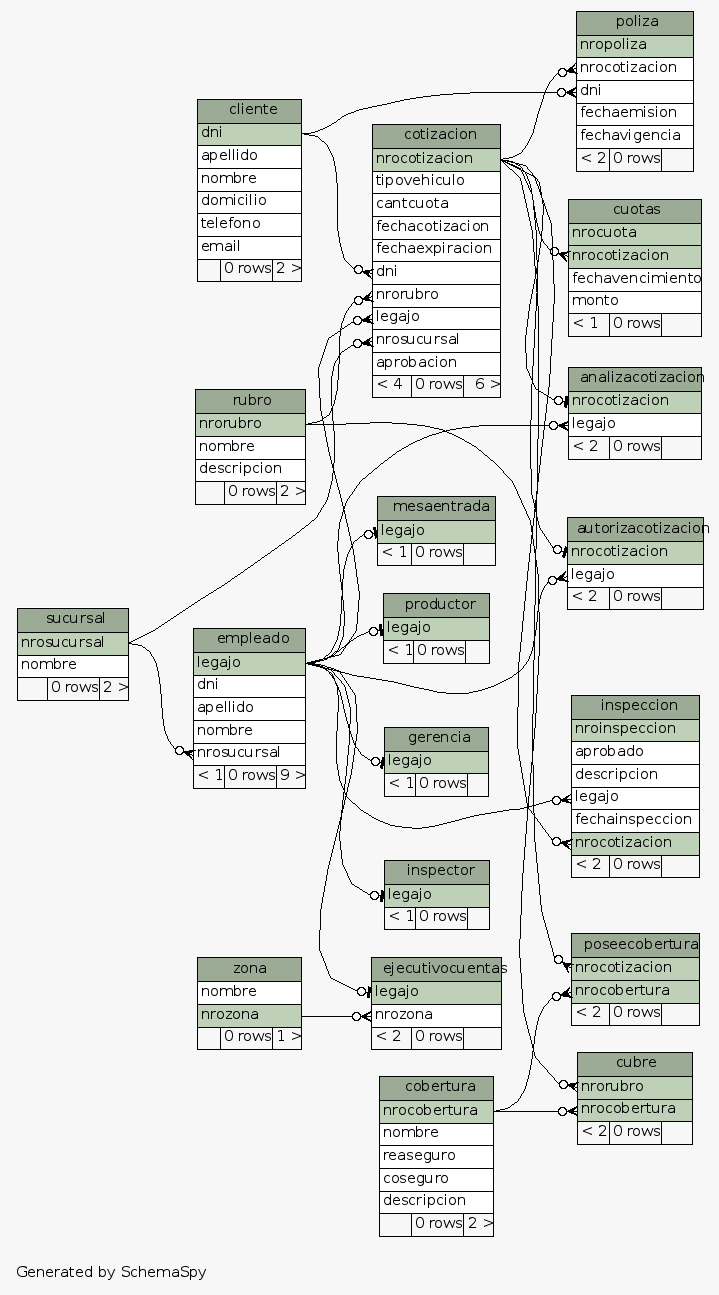
\includegraphics[width=15cm,height=25cm,angle=0]{build/images/rel2.png}
	\caption{Modelo relacional} \label{fig:relacional}
\end{figure}

\FloatBarrier

\subsection{Scripts de creación}

%A continuación se incluyen los scripts de creación de las tablas del modelo
%relacional para ser ejecutado en un sistema de bases de datos que interprete
%SQL, particularmente las instrucciones DDL de dicho lenguaje. No se incluyen
%las instrucciones, normalmente específicas al motor propiamente dicho, de
%creación de usuarios, roles, schemas y bases de datos correspondientes.

\lstinputlisting[inputencoding=latin1,language=SQL,caption={Script de definición de la base de datos}]{../scripts/script_creacion_db.sql}

\clearpage

\part{Apéndice}
\appendix

\section{Enunciado original}\label{sec:enunciado}
\includepdf[pages={-}, frame=true, pagecommand={}, noautoscale=true, scale=0.7]{doc/enunciado.pdf}

\end{document}

